\chapter{Implementierung}
\section{Implementierung des Sprachverarbeitungssystems}\label{section:Implementierung_Sprachverarbeitung}
\subsection{Word2Vec-Modell}
\subsection{Sequence-to-Sequence-Modell}
\section{Implementierung der Sprachsteuerung}
Im Folgenden wird erläutert, wie die Sprachsteuerung für die Getränkemischmaschine implementiert wurde und welche Technologien dafür zum Einsatz kamen. Dabei wird zunächst auf die Spracherkennung d.h., die Umwandlung der Audiosignale (Sprachbefehl des Benutzers) in eine Form, die innerhalb des Quelltextes weiterverarbeitet werden kann, eingegangen (s. Abschnitt \ref{section:Spracherkennung}). Danach wird die Anbindung des Sprachverarbeitungssystems beschrieben, dessen Implementierung in Abschnitt \ref{section:Implementierung_Sprachverarbeitung} erklärt wird. Abschließend wird die Kommunikation mit der Mischmaschine über den Arduino illustriert (s. Abschnitt \ref{section:Befehlsverarbeitung}).
\subsection{Spracherkennung}\label{section:Spracherkennung}
Die Spracherkennung ist der erste Schritt bei der Implementierung einer Sprachsteuerung für die Getränkemischmaschine. Mit Spracherkennung ist die Aufnahme eines Tonsignals über ein Audio-Eingabegerät (Mikrofon) und die Umwandlung der Audiodaten in Text gemeint. Der Quelltext zur Implementierung der Sprachsteuerung erfolgt mit der Programmiersprache \textit{Python}, da hier sehr viele, leicht zu bedienende Bibliotheken zur Spracherkennung, -verarbeitung und \ac{KI} zur Verfügung stehen.\\\\
Für dieses Projekt viel die Wahl auf das Paket \textit{SpeechRecognition}, das die Verwendung verschiedener Spracherkennungsdienste über eine einheitliche Schnittstelle ermöglicht und zu diesem Zweck auch zur Aufnahme und Verarbeitung der Audiosignale verwendet werden kann \cite{speechrecognition}. Ein großer Vorteil davon ist, dass dadurch ein schneller Wechsel der eingesetzten \ac{API} erfolgen kann, sollte dies erforderlich sein. Die Verwendung des \textit{SpeechRecognition}-Pakets findet fast ausschließlich über die \textit{Recognizer}-Klasse statt. Um Audiosignale über eine physische Audioquelle (bspw. ein Mikrofon am Computer) aufzunehmen kann die \textit{Microphone}-Klasse verwendet werden, die ebenfalls im Paket enthalten ist. Mit Hilfe eines Objekts vom Typ \textit{Microphone} und der Methode \textit{listen} der \textit{Recognizer}-Klasse können anschließend Audiodaten aufgenommen werden, die in einem Objekt vom Typ \textit{AudioData} gespeichert sind. Die Verwendung von \textit{Recognizer} und \textit{Microphone} sind in Listing \ref{speech_rec_1} zu sehen. 
\lstinputlisting[language=python, style=algoBericht, label={speech_rec_1}, basicstyle=\tiny\sffamily, captionpos=b, caption={Audioaufnahme mit \textit{SpeechRecognition}}]{./Listings/speech_rec_1.py}
Das \textit{AudioData}-Objekt kann nun verwendet werden um die darin gespeicherten Audiodaten zu erkennen und in Text umzuwandeln. Das \textit{SpeechRecognition}-Paket stellt dafür verschiedene Möglichkeiten zur Verfügung, wie eingangs erwähnt wurde. Diese sollen im Folgenden kurz beschrieben werden:
\begin{itemize}
    \item Whisper: Whisper ist ein neuronales Netz das von der Firma \textit{OpenAI} trainiert und als Open-Source-Projekt zur Verfügung gestellt wird \cite{openai,whisper}. Neben der Fähigkeit Sprache in Text zu konvertieren kann es auch eingesetzt werden um Transkripte zu generieren, die gesprochene Sprache automatisch zu erkennen oder in die englische Sprache zu übersetzen. Das Paket \textit{SpeechRecognition} lässt sowohl die Verwendung der von \textit{OpenAI} zur Verfügung gestellten Online-\ac{API} zu, als auch die lokale Ausführung des Sprachmodells. Aufgrund der Anforderung nach Offline-Funktionalität entfällt die erste Möglichkeit (s. Kapitel \ref{chap:Anforderungen}).
    \item Sphinx: Das \textit{CMUSphinx} Projekt wird von der \ac{CMU} unterhalten und stellt eine Reihe von Werkzeugen und Bibliotheken zur Spracherkennung zur Verfügung \cite{sphinx_about}. Darunter fallen bspw. \textit{PocketSphinx}, \textit{SphinxTrain} und \textit{sphinx4}. Bei \textit{PocketSphinx} handelt es sich um eine C-Bibliothek zur Spracherkennung, die auch innerhalb von Python verwendet werden kann. \textit{SphinxTrain} hingegen stellt Ressourcen zum Trainieren eigener Modelle bereit. \textit{sphinx4} ist das Java-Equivalent zu \textit{PocketSphinx}. Somit ist für dieses Projekt nur \textit{PocketSphinx} interessant. Leider unterstützt enthält das Paket standardmäßig nur ein Modell für die englische Sprache. Anderssprachige Modelle und weitere dazugehörige Ressourcen müssen mühsam aus externen Quellen bezogen und eingebunden werden.
    \item Snowboy: \textit{Snowboy Hotword Detection} ist ein quelloffenes Projekt welches Bibliotheken für verschiedene Programmiersprachen bereitstellt, die dem Erkennen sog. \glqq{}hot words\grqq{} dienen \cite{snowboy}. Ein \textit{hot word} sind ein oder mehrere Wörter die der Aktivierung eines Sprachsteuerungssystems dienen. Bekannte Beispiele hierfür sind \glqq{}Alexa\grqq{} oder \glqq{}OK Google\grqq{}. Das System \glqq{}hört\grqq{} im Hintergrund und wartet darauf, dass das \textit{hot word} genannt wird. Anschließend nimmt das System weitere Sätze, die vom Benutzer gesprochen werden, wahr und verarbeitet diese. Ein \textit{hot word} ist notwendig damit das System nicht dauerhaft versucht Sätze zu verarbeiten, die nicht für das System gedacht sind und damit wiederholt Fehler bekommt oder unerwünschtes Verhalten an den Tag legt. Da die Ansprüche des vorliegenden Projekts an die Detektion von \textit{hot words} nicht besonders hoch sind und um die von Snowboy benötigte Rechenzeit einzusparen wird \textit{Snowboy} in diesem Projekt keine Relevanz haben. Auf die konkrete Umsetzung des \textit{hot word} Mechanismus wird später noch eingegangen. Ein weiterer Grund dafür, dass Snowboy nicht zum Einsatz kommen soll ist, dass das Projekt bereits im Jahr 2020 offiziell eingestellt wurde und nur noch von der Community weiter betrieben wird. 
    \item Vosk: Das \textit{Vosk Speech Recognition Toolkit} ist neben \textit{Whisper} und \textit{Sphinx} die dritte und letzte verfügbare offline \ac{API} für die \textit{SpeechRecognition} eine Schnittstelle bereitstellt \cite{vosk,vosk_repo}. Es wird von der \textit{Alpha Cephei Incorporation} vertrieben. Ähnlich wie bei Whisper sind vortrainierte Modelle in vielen verschiedenen Sprachen bereits vorhanden, müssen allerdings manuell heruntergeladen und dem \textit{SpeechRecognition} Paket zur Verfügung gestellt werden.
    \item Google: \textit{SpeechRecognition} bietet zwei Möglichkeiten Google-Dienste zur Konvertierung von Sprache zu Text zu verwenden. Die erste Möglichkeit besteht in der Verwendung der \textit{Google Speech API} in der \textit{Google Cloud} \cite{google_cloud_speech}. Die zweite Möglichkeit besteht in der Verwendung der \textit{Google Speech API} ohne die \textit{Google Cloud}. Die Verwendung der Google-Schnittstelle entfällt jedoch für dieses Projekt, da eine aktive Internetverbindung Voraussetzung dafür ist. Außerdem sind die Google-Dienste weder kostenfrei noch open-source.
    \item Microsoft: Auch hier gibt es zwei verschiedene Möglichkeiten Microsoft-Dienste zur Umwandlung von Sprache zu Text über das \textit{SpeechRecognition}-Paket zu nutzen. Eine davon ist die Verwendung der \textit{Speech to text} Funktion in der \textit{Microsoft Azure Cloud} \cite{azure_speech_to_text}. Hierfür sind ein aktiver \textit{Azure}-Account sowie ein gültiger \ac{API}-Schlüssel notwendig. Die zweite Möglichkeit besteht in der \textit{Microsoft Bing Voice Recognition}. Diese ist jedoch veraltet und wird nicht mehr unterstützt. Auch diese Schnittstelle enfällt jedoch wegen der notwendigen Internetverbindung und Bezahlung. 
    \item IBM: Auch die Firma IBM bietet ihre eigene Schnittstelle zur Spracherkennung mit Hilfe der von IBM entwickelten \ac{KI} \textit{Watson} an \cite{ibm_speech_to_text}. Auch hier gilt: zur Verwendung der \ac{API} ist sowohl eine aktive Internetverbindung als auch Bezahlung vorgesehen, weshalb diese Schnittstelle für das Projekt nicht in Frage kommt.
    \item Weitere Schnittstellen sind \textit{Wit.ai}, \textit{Houndify} und \textit{Tensorflow} \cite{witai,houndify,tensorflow_home}. Da diese Schnittstellen allderdings ebenso eine aktive Internetverbindung voraussetzen und damit ausscheiden soll nicht weiter auf sie eingegangen werden.
\end{itemize}
Die einzelnen \ac{API}s lassen sich jeweils über einen Methodenaufruf der Form \textit{Recognizer.recognize\_x} verwenden, wobei das \glqq{}x\grqq{} für den Namen der jeweiligen \ac{API} steht. Für dieses Projekt viel die Wahl auf die Verwendung der \textit{Whisper}-Bibliothek von \textit{OpenAI}. Dies ist damit zu begründen, dass sie von den offline verwendbaren \ac{API}s die mit Abstand am einfachsten zu verwendende ist und gleichzeitig sehr gute Ergebnisse beim Testen damit erzielt wurden. Beispielsweise werden die Modelle für viele verschiedene Sprachen bereits von OpenAI zur Verfügung gestellt und für jedes Modell stehen weitere Ausführungen zur Verfügung die nach den eigenen Ansprüchen und vorhandenen Ressourcen ausgewählt werden können. Die verschiedenen Ausführungen sind nach der \glqq{}Größe\grqq{} des Modells unterteilt in \glqq{}tiny\grqq{}, \glqq{}base\grqq{}, \glqq{}small\grqq{}, \glqq{}medium\grqq{} und \glqq{}large\grqq{} \cite{whisper_repo}.
\lstinputlisting[language=python, style=algoBericht, label={speech_rec_2}, basicstyle=\tiny\sffamily, captionpos=b, caption={Sprache zu Text mit \textit{OpenAI Whisper}}]{./Listings/speech_rec_2.py}
Listing \ref{speech_rec_2} zeigt, wie mit Hilfe der \textit{Whisper}-\ac{API} die aufgenommenen Audiodaten zu Text verarbeitet und ausgegeben werden können. Die Sprache und die Modellgröße werden bei dem Methodenaufruf \textit{Recognizer.recognize\_whisper} angegeben. Sollte das entsprechende Modell noch nicht lokal vorliegen wird dieses bei der ersten Ausführung automatisch installiert, was einen hohen Grad an Benutzerfreundlichkeit seitens der \ac{API} bedeutet. 
\subsubsection{Herausforderungen bei der Implementierung der Spracherkennung}
Die Verwendung von \textit{Whisper} setzt die Installation von \textit{PyTorch} voraus - einem quelloffenen \ac{ML}-Framework \cite{pytorch}. Die Installation von \textit{PyTorch} kann auf zwei unterschiedlichen Wegen erfolgen:
\begin{enumerate}
    \item Unter der Benutzung vorkompilierter Distributionen mit Hilfe eines Paketverwaltungssystems wie etwa \textit{pip} \cite{pip}.
    \item Durch das eigenständige Bauen des Quelltextes auf dem lokalen Rechner.
\end{enumerate}
Da es sich bei \textit{PyTorch} um ein überaus großes und komplexes Projekt handelt ist es empfehlenswert die erste Methode anzuwenden, da der Build-Vorgang bei Methode zwei sehr viele Ressourcen benötigt.\\\\
Nach der Verwendung von \textit{pip} zur Installation von \textit{PyTorch} auf dem für das Projekt verwendeten \textit{Raspberry Pi 4B} kam es jedoch zu einem unerwarteten Fehler. Das Importieren der \textit{PyTorch}-Bibliothek ließ das Programm sofort beenden und die Nachricht \glqq{}Illegal Instruction\grqq{} auf dem Bildschirm ausgeben. Die Fehlermeldung lässt darauf schließen, dass die Bibliothek einen für den Prozessortyp unbekannten Befehl ausüben will. Drei Lösungsansätze wurden daraufhin konzipiert:
\begin{enumerate}
    \item Das Programm sollte mit einer anderen Python-Version ausgeführt werden.
    \item Das vorkompilierte Paket, das automatisch von \textit{pip} ausgewählt wurde scheint nicht auf die vorhandene Prozessorarchitektur zu passen und führt unbekannte Maschinenbefehle aus. Deshalb sollte die \textit{PyTorch}-Bibliothek selbstständig, lokal kompiliert werden.
    \item Ein anderes vorkompiliertes Paket herunterladen und installieren, das auf die vorhandene Prozessorarchitektur angepasst und optimiert ist.
    \item Sollten alle zuvor genannten Versuche scheitern muss \textit{Whisper} durch eine andere Bibliothek ersetzt werden, die keine Abhängigkeit zu \textit{PyTorch} aufweist.
\end{enumerate}
Lösungsansatz eins erwies sich als nicht effektiv. Das Programm verursachte immernoch den selben Fehler. Lösungsansatz zwei scheiterte, da der Build-Prozess mehr als den zur Verfügung stehenden \ac{RAM} des Raspberry Pi aufbrauchte. Sogar mit vier \ac{GB} zusätzlich konfiguriertem Swap-Speicher wurde der Build-Prozess nach einiger Zeit vom Betriebssystem beendet aufgrund des hohen \ac{RAM}-Verbrauchs. Lösungsansatz drei funktionierte schließlich. Mit Hilfe des vorkompilierten Pakets aus \cite{q-engineering_install_nodate} konnte \textit{PyTorch} installiert und erfolgreich importiert und verwendet werden.\\\\
Ein weiteres Problem trat bei der Verwendung des Mikrofons über die \textit{SpeechRecognition}-Bibliothek auf. Bei den Aufrufen \textit{speech\_recognition.Microphone()} und\\ \textit{speech\_recognition.Recognizer().listen(source)} kommt es auf dem Raspberry Pi zu unerwarteten Fehlermeldungen, die in Abbildung \ref{img:alsa_errors} zu sehen sind.
\begin{figure}[H]
    \centering
    \fbox{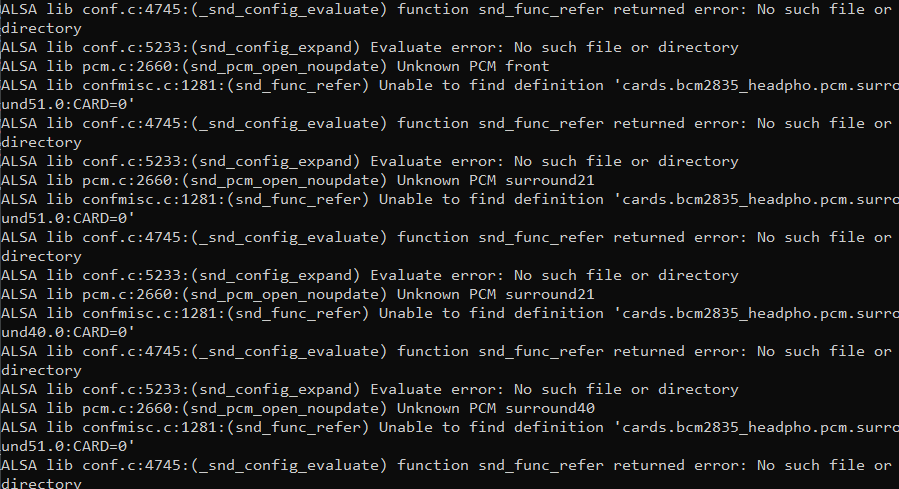
\includegraphics[width=0.8\textwidth]{./img/Bilder_Implementierung/alsa_errors.png}}
    \caption{Fehlermeldungen beim Zugriff auf das Mikrofon}
    \label{img:alsa_errors}
\end{figure}
\noindent
Zwar kann das Programm trotz der Meldungen fehlerfrei ausgeführt werden, jedoch stören die Meldungen bspw. beim Debuggen und irritieren evtl. Programmierer, die zu einem späteren Zeitpunkt einen Blick auf das Projekt werfen. Um die Fehlermeldungen zu umgehen wurde deshalb im finalen Quelltext die Fehlerbehandlungsfunktion der \textit{libasound}-Bibliothek ausgetauscht wie in Listing \ref{speech_rec_3} zu sehen ist.
\lstinputlisting[language=python, style=algoBericht, label={speech_rec_3}, basicstyle=\tiny\sffamily, captionpos=b, caption={Fehlerbehandlung}]{./Listings/speech_rec_3.py}
Für einen Vorher-/Nachher-Vergleich sei auf Listing \ref{speech_rec_2} verwiesen. Zeilen vier bis zehn dienen der Definition einer C-Funktion zur Fehlerbehandlung, die bei ihrer Ausführung die auftretende Meldung ignoriert. In Zeile 16 wird die Standard Fehlerfunktion durch diese ersetzt und in Zeile 19 wieder zurückgeändert. 
\subsection{Anbindung des Sprachmodells an die Mischmaschine}
\subsection{Befehlsverarbeitung in der Mischmaschine}\label{section:Befehlsverarbeitung}
Nachdem die Sprache des Benutzers erkannt, in Text konvertiert und durch das Sprachmodell interpretiert wurde muss der zurückerhaltene Befehl vom Raspberry Pi and den Arduino in der Getränkemischmaschine gesendet werden. Zur Umsetzung der Kommunikation zwischen Raspberry Pi und Arduino kommt die \textit{PySerial}-Bibliothek zum Einsatz \cite{pyserial}. Listing \ref{serial_1_py} zeigt, wie die Bibliothek zum Versenden von Nachrichten an ein Gerät über die serielle Schnittstelle erfolgen kann.
\lstinputlisting[language=python, style=algoBericht, label={serial_1_py}, basicstyle=\tiny\sffamily, captionpos=b, caption={Serielle Kommunikation in Python}]{./Listings/serial_1.py}
Das Programm öffnet in Zeile vier die serielle Schnittstelle zu dem Gerät mit dem Namen \glqq{}ttyACM0\grqq{}, mit einer Baud-Rate von 9600 und einem Timeout von fünf Sekunden. Der Gerätename ist je nach Gerät und Betriebssystem unterschiedlich und muss zuvor mit den verfügbaren Betriebssystemmitteln bestimmt werden. Die Baud-Rate gibt an, mit welcher Geschwindigkeit Symbole über die Schnittstelle gesendet werden. Die Baud-Rate muss sowohl beim Sender als auch beim Empfänger gleich sein, da es sonst zu Kommunikationsproblemen kommt. Der Timeout steuert wie lange bei einer Leseoperation gewartet werden soll, bis alle zu lesenden Bytes im Puffer vorhanden sind.\\\\
In der darauffolgenden Zeile wird der Eingabepuffer geleert, um zu verhindern, dass unvollständige Daten an den Empfänger gesendet werden, die beim letzten Programmdurchlauf im Puffer verblieben sein könnten. Da der Verbindungsaufbau mit dem Gerät einige Zeit dauern kann wird die Programmausührung in Zeile sechs zunächst um fünf Sekunden verzögert.\\\\
In Listing \ref{serial_1_ino} ist der Quelltext auf Empfängerseite zu sehen.
\lstinputlisting[language=c++, style=algoBericht, label={serial_1_ino}, basicstyle=\tiny\sffamily, captionpos=b, caption={Serielle Kommunikation in Python}]{./Listings/serial_1.ino}
\subsubsection{Herausforderungen bei der Implementierung der Befehlsverarbeitung}
\endinput


